% An annulus X with a 1-chain c (three arcs v0->v1->v2->v0) circling the hole.
% Source: book/tex/homology/singular.tex (§ The singular homology groups).
\documentclass[border=2mm]{standalone}
\usepackage{tikz}
\usetikzlibrary{arrows.meta}
\begin{document}
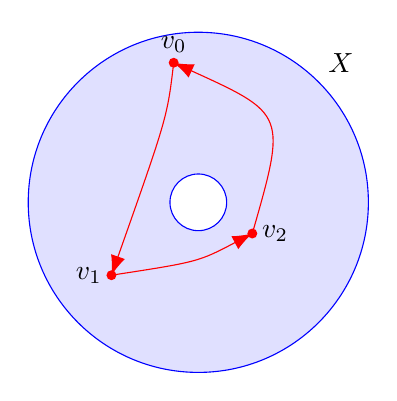
\begin{tikzpicture}[>={Latex[length=2.5mm]}, scale=0.36]
  \fill[blue!12] (0,0) circle (6);
  \fill[white] (0,0) circle (1);
  \draw[blue] (0,0) circle (6);
  \draw[blue] (0,0) circle (1);
  \node[above right] at ({6*cos(45)},{6*sin(45)}) {$X$};
  \coordinate (v0) at ({5*cos(100)},{5*sin(100)});
  \coordinate (v1) at ({4*cos(220)},{4*sin(220)});
  \coordinate (v2) at ({2.2*cos(330)},{2.2*sin(330)});
  \draw[red, ->] (v0) .. controls ({3.2*cos(110)},{3.2*sin(110)}) .. (v1);
  \draw[red, ->] (v1) .. controls ({2.1*cos(270)},{2.1*sin(270)}) .. (v2);
  \draw[red, ->] (v2) .. controls ({4.4*cos(45)},{4.4*sin(45)}) .. (v0);
  \fill[red] (v0) circle (5pt); \node[above] at (v0) {$v_0$};
  \fill[red] (v1) circle (5pt); \node[left] at (v1) {$v_1$};
  \fill[red] (v2) circle (5pt); \node[right] at (v2) {$v_2$};
\end{tikzpicture}
\end{document}
